\documentclass{article}

\usepackage{fancyhdr}
\usepackage{extramarks}
\usepackage{amsmath}
\usepackage{amsthm}
\usepackage{amsfonts}
\usepackage{tikz}
\usepackage[plain]{algorithm}
\usepackage{algpseudocode}

\usetikzlibrary{automata,positioning}

%
% Basic Document Settings
%

\topmargin=-0.45in
\evensidemargin=0in
\oddsidemargin=0in
\textwidth=6.5in
\textheight=9.0in
\headsep=0.25in

\linespread{2.0}

\pagestyle{fancy}
\lhead{\hmwkAuthorName}
\chead{\hmwkClass\ (\hmwkClassInstructor\ \hmwkClassTime)}
\rhead{\firstxmark}
\lfoot{\lastxmark}
\cfoot{\thepage}

\renewcommand\headrulewidth{0.4pt}
\renewcommand\footrulewidth{0.4pt}

\setlength\parindent{0pt}

%
% Create Problem Sections
%

\newcommand{\enterProblemHeader}[1]{
    \nobreak\extramarks{}{Problem \arabic{#1} continued on next page\ldots}\nobreak{}
    \nobreak\extramarks{Problem \arabic{#1} (continued)}{Problem \arabic{#1} continued on next page\ldots}\nobreak{}
}

\newcommand{\exitProblemHeader}[1]{
    \nobreak\extramarks{Problem \arabic{#1} (continued)}{Problem \arabic{#1} continued on next page\ldots}\nobreak{}
    \stepcounter{#1}
    \nobreak\extramarks{Problem \arabic{#1}}{}\nobreak{}
}

\setcounter{secnumdepth}{0}
\newcounter{partCounter}
\newcounter{homeworkProblemCounter}
\setcounter{homeworkProblemCounter}{1}
\nobreak\extramarks{Problem \arabic{homeworkProblemCounter}}{}\nobreak{}

%
% Homework Problem Environment
%
% This environment takes an optional argument. When given, it will adjust the
% problem counter. This is useful for when the problems given for your
% assignment aren't sequential. See the last 3 problems of this template for an
% example.
%
\newenvironment{homeworkProblem}[1][-1]{
    \ifnum#1>0
        \setcounter{homeworkProblemCounter}{#1}
    \fi
    \section{Problem \arabic{homeworkProblemCounter}}
    \setcounter{partCounter}{1}
    \enterProblemHeader{homeworkProblemCounter}
}{
    \exitProblemHeader{homeworkProblemCounter}
}

%
% Homework Details
%   - Title
%   - Due date
%   - Class
%   - Section/Time
%   - Instructor
%   - Author
%

\newcommand{\hmwkTitle}{Homework\ \#3}
\newcommand{\hmwkDueDate}{September 11th, 2015}
\newcommand{\hmwkClass}{Differential Equation}
\newcommand{\hmwkClassTime}{Section 061}
\newcommand{\hmwkClassInstructor}{Professor Heather Lee}
\newcommand{\hmwkAuthorName}{Yao Xiao}

%
% Title Page
%

\title{
    \vspace{2in}
    \textmd{\textbf{\hmwkClass:\ \hmwkTitle}}\\
    \normalsize\vspace{0.1in}\small{Due\ on\ \hmwkDueDate\ at 3:10pm}\\
    \vspace{0.1in}\large{\textit{\hmwkClassInstructor\ \hmwkClassTime}}
    \vspace{3in}
}

\author{\textbf{\hmwkAuthorName}}
\date{}

\renewcommand{\part}[1]{\textbf{\large Part \Alph{partCounter}}\stepcounter{partCounter}\\}

%
% Various Helper Commands
%

% Useful for algorithms
\newcommand{\alg}[1]{\textsc{\bfseries \footnotesize #1}}

% For derivatives
\newcommand{\deriv}[1]{\frac{\mathrm{d}}{\mathrm{d}x} (#1)}

% For partial derivatives
\newcommand{\pderiv}[2]{\frac{\partial}{\partial #1} (#2)}

% Integral dx
\newcommand{\dx}{\mathrm{d}x}

% Alias for the Solution section header
\newcommand{\solution}{\textbf{\large Solution}}

% Probability commands: Expectation, Variance, Covariance, Bias
\newcommand{\E}{\mathrm{E}}
\newcommand{\Var}{\mathrm{Var}}
\newcommand{\Cov}{\mathrm{Cov}}
\newcommand{\Bias}{\mathrm{Bias}}

\begin{document}

\maketitle

\pagebreak

\begin{homeworkProblem}
1. \\
\(xdx+ye^{-x}dy=0\)

\(xe^xdx=-ydy \)

\(e^{x}(x-1)=-\frac{1}{2}y^2 + C \)

\( -1 = -\frac{1}{2}+C\)

\( C=-\frac{1}{2} \)

\(2e^{x}(1-x)=y^2+1\)

\(y=\sqrt{2e^{x}(1-x)-1} \)

2.\\
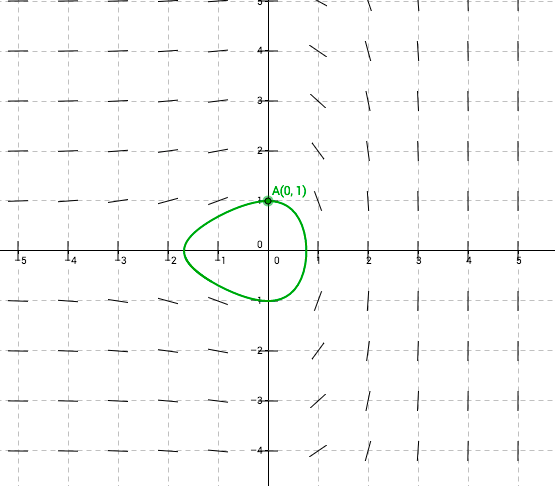
\includegraphics[scale=0.5]{image1.png}  \\

3.  Since the function will become vertical at around 0.7 and -1.7, so it would be valid when \( -1.7<x<0.7 \)
\end{homeworkProblem}

\begin{homeworkProblem}
\(y' = xy^3(1+x^2)^{-1/2}\) \\
1. \[
\begin{split}
\frac{dy}{dx}&=xy^3(1+x^2)^{-1/2}\\
y^{-3}dy&=x(1+x^2)^{-1/2}dx \\
-\frac{1}{2}y^{-2} &= \sqrt{x^2+1} +C \\
\end{split}
\] 
When x=0, y=1
\(1+C=-1/2, \ C=-3/2 \) \\
\(y^{-2}=-2\sqrt{x^2+1}+3 \) \\
\(y=(-2\sqrt{x^2+1}+3)^{-1/2} \) \\
2. \\
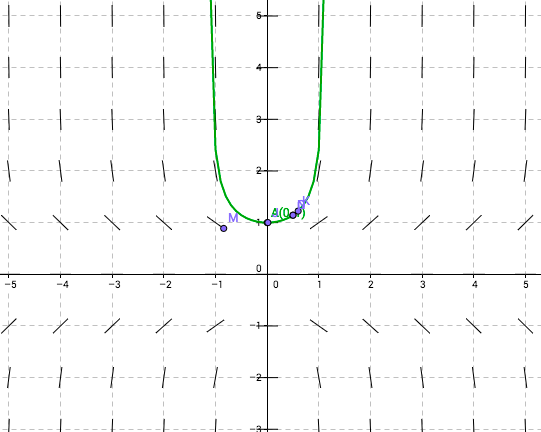
\includegraphics[scale=0.5]{image2.png}  \\
3. \\ We need to make sure \(-2\sqrt{x^2+1}+3\neq 0\)
So \(x\neq \frac{1}{2}\sqrt{5} \), since x=0 should be in the interval,  the answer would be \( -\frac{1}{2}\sqrt{5}<x<\frac{1}{2}\sqrt{5}
\)

\end{homeworkProblem}


\begin{homeworkProblem}
1. When \( t \to \infty \), \(\frac{t}{1+t} \to 1\) , \(y'=y(4-y)=0 \), also \(y\neq 0\) so \(y \to 4\)\\
2. \[
\begin{split}
dy/(y*(4-y)) &= t/(1 + t) dt  \\
ln(y)- ln(4 - y) &= 4t - 4 ln (1 + t) + C \\
ln\frac{4}{4-y} &= 4t-4ln(1+t)+C \\
\frac{y}{4-y} &= \frac{Ce^{4t}}{(1+t)^4}
\end{split}
\]
If \(y_0 = 2 \) \( C=1 \) and we plug in \(y=2\) we get  \(3.99/(4-3.99) = e^{4t}/(1+t)^4\), \(t=2.84\) \\
3. I don't know...

\end{homeworkProblem}

\begin{homeworkProblem}
1.\\ \((x^2+3xy+y^2)dx-x^2dy=0\) is equal to
\(v=y/x, (v^2+3v+1)dx-1dy=0, v^2+3v+1=\frac{dy}{dx} \) So it's homogeneous. \\
2.\\ \[ 
\begin{split}
v+x\frac{dv}{dx} &= v^2+3v+1 \\
			\frac{dv}{dx} &=(v+1)^2 \\			
			ln(x) + (v+1)^{-1} +C &= 0 \\
			ln(x)+(y/x+1^{-1})+C &= 0 \\
		\end{split}		
\] \\

3. \\
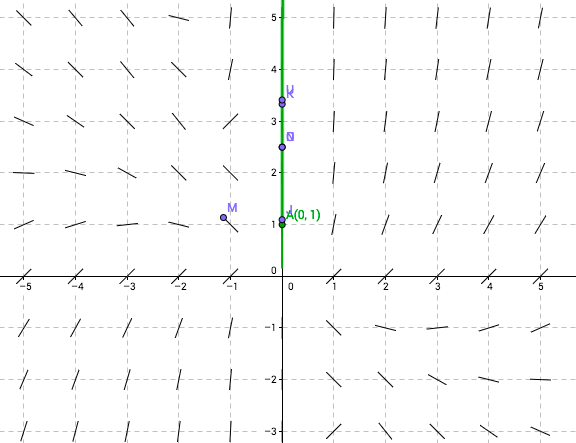
\includegraphics[scale=0.5]{image3.png}  \\
It's not symmentric

\end{homeworkProblem}

\begin{homeworkProblem}
\[
\begin{split}
u &= x+y \\
u' &= x'+y' = 1+y' \\
u' &= u^2+1 \\
x=tan^{-1}(u)+C \\
x=tan^{-1}(x+y)+C
\end{split}
\]
\end{homeworkProblem}


\begin{homeworkProblem}
\[
\begin{split}
\frac{du}{dx}=3y^2dy/dx \\
 1/3 * du/dx + u(x)/x = 2/x^2 \\
 x^3*u = 3x^2 + C \\
 (xy)^3 = 3x^2 + C
\end{split}
\]
\end{homeworkProblem}


\begin{homeworkProblem}
Q(t) means the amount of dye in the tank at time t, the system lost  2 L/min *(Q(t)/200) g/L = Q(t)/100 g/min
\[
\begin{split}
\frac{dQ}{dt} = -0.01Q
\end{split}
\]
Also Q(0)=200g
So \(Q(t) = 200e^{-0.01t} \) \\
when \( 200e^{-0.01t} = 2 \) , t=460.5min
\end{homeworkProblem}



\begin{homeworkProblem}

\end{homeworkProblem}

\end{document}
